\chapter{Something about strained hBN}
\chaptertoc{}

\section{oui}
\textit{This chapter is partly based on our publication \cite{lechifflart2022excitons}. Some of the text and figures contained in this Chapter are adapted from this reference. }
\begin{itemize}
	\item in the intro, talk about strain-induced symmetry breaking
	\item experimental motivations
	\item why we build the orthorombic cell 
	\item relaxation of the structures (I didn't mention structure relaxtion with DFT anywhere)
	\item convert orthorombic to pseudo-hexagonal (this could be an appendix)
	\item alot of computational details
	\item electronic band structure 
	\item exciton-phonon coupling from finite differences
	\item vRS relation in this case 
\end{itemize}
%
%
ETSF webinar of Fulvio
indirect bandgap only; we can write the response function with derivatives of the response function because we consider only phonon-assisted transitions; need supercells
converge the displacement so that it is the smallest possible
PLE (propto absorption) or absorption and PL are not symmetric, as expected for direct gaps
the minimum exciton at T is the degenerate dark state at Gamma which splits
for absorption, the bright exciton overlaps with the phonon replicas and it is so bright that we don't see them 

%
\section{Experimental motivations}
From Léonard Schué's thesis, (suspended nanosheet of hBN), they conclude that there is probably a residual uniaxial strain at the center of the suspended sheet. They use cathodoluminescence, where the electron beam penetrates in the bulk of the crystal

In this experiment, the group of Julien Barjon, specifically Léonard Schué, they suspended a nanosheet of hexagonal Boron Nitride on a over a trench carved out from an SiO$_2$ substrate. The nanosheet is about 100 nm thick and curves under the effect of gravity, as illustrated in Fig. \ref{fig:exp_strain}(a), and was imaged by \acrfull{AFM} (Fig. \ref{fig:exp_strain}(b)).
\begin{figure}[h!tbp]
	\vspace{0.5cm}
	\setcapindent{2em}
	\centering
	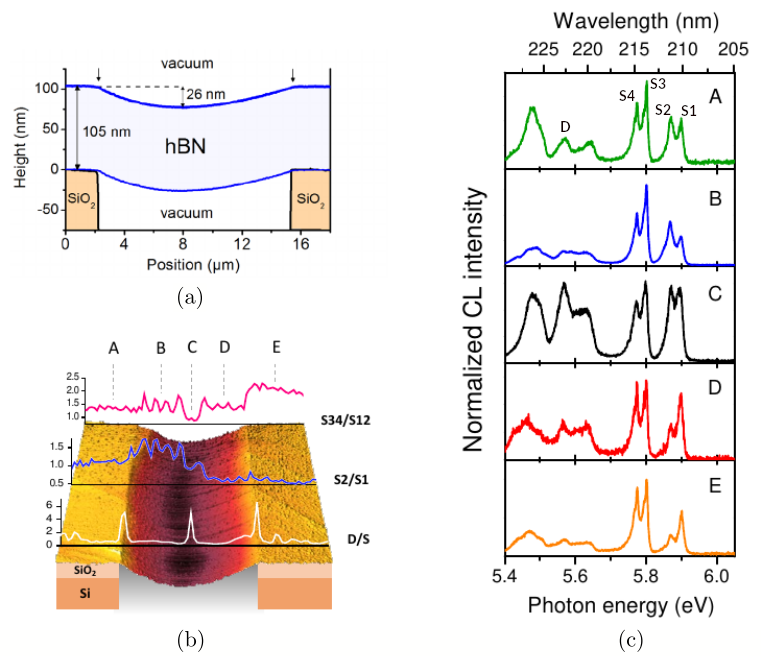
\includegraphics[width=0.8\textwidth]{exp_strain.png}
	\caption{(a) Sketch of the deposited hBN nanosheet on the trench. (b) AFM profile and relative intensity ratios of different emission peaks with respect to spatial region. (c) Cathodoluminescence intensity measured on different regions of the sample. \textcolor{red}{Courtesy of Léonard Schué and Julien Barjon}}
	\label{fig:exp_strain}
\end{figure}
When measuring the cathodoluminescence spectra at different positions on the sample, one can see that the intensity ratios between different peaks are varying. Their interpretation is that the deformation of the sample induces uniaxial (compressive) strain, perpendicular to the trench. This strain could have an effect on the recombination process of excitons, leading to a change in the luminescence intensity. \textcolor{red}{elaborate a bit more : give ratio values for instance and say that regions have more defects}
%
%
\section{Structure and phonons}
In order to simulate the hBN sample in suspension, we simulate (\textcolor{green}{meh}) an infinite bulk crystal under uniaxial strain. In the experiment, the beam of electron penetrates only on the upper part of the nanosheet, where the strain is compressive. However for the first steps of the computational workflow, we study a range of strain including both stretching and compression around the equilibrium structure.
First, we obtain the strained structure by taking an orthorombic cell of the pristine crystal, larger than the hexagonal unit cell. Because it has three orthogonal lattice vectors, the orthorombic cell is more suited for the application of a uniaxial strain. To do so, we simply alter the length of one cell vector, up to an arbitrary length corresponding to a value of strain. We studied different strain values, in an interval going from a $+2.5\%$ to a $-2.5\%$ variation of the equilibrium length. In this work we applied strained in the armchair direction, the one parallel to the B-N bond. \textcolor{red}{include the figure here}
After setting the length of the cell to the desired length corresponding to a strain value, we let the atom positions and the other two cell vectors relax, using a damped molecular dynamics algorithm where the forces acting on the atoms are computed in \acrshort{DFT} using the Hellmann--Feynman theorem. This procedure in implemented in the \qe ~suite \cite{giannozzi2009quantum,giannozzi2017advanced}. More computational details can be found in Appendix \ref{app:comp_par_strain} \textcolor{red}{write it}. We found that once the two cell vectors orthogonal to the strained one are relaxed, their length vary linearly with the strain.\\
Once we have the relaxed strained orthorombic cells, we want to construct a pseudo-hexagonal unit cell containing only four atoms. This way, we can compare the structures obtained for different strain values with the equilibrium structure in a consistent way and proceed with the calculation of electronic and optical properties. To construct the pseudo-hexagonal cells from the strained orthorombic ones, we followed the procedure described in Appendix \ref{app:ortho2hex}. We computed the phonon-related properties using \acrshort{DFPT} in the four-atom strained cells. In the strained crystal, whatever the value of strain, the 120\textdegree~ rotational symmetry is broken and this makes the \MM~and \KK~points in the \acrshort{BZ} inequivalent to the \MM' and \KK' points. The path between high-symmetry points containing all four of these points is drawn in yellow in Fig. \textcolor{red}{the figure 3 ?}.
The resulting phonon dispersions are shown in Fig. \textcolor{red}{put the figure}, for three strain values : a $+2.5\%$ stretch, a $-2.5\%$ compression and the equilibrium one. 
For the unstrained dispersion we can notice the splitting of the highest branch at $\Gamma$ with the two branches below. This is the LO-TO splitting mentionned in Sec. \ref{sec:DFPT}.

We found that the optical modes (the branches with the highest energies) are the most affected by strain. With compressive strain, their frequencies are increased at all $\qq$ points and they are decreased for tensile strain. We also observe the splitting of the E$_{2g}$ modes, whose frequencies are degenerate at $\Gamma$ just below 175 meV or 1400 cm$^{-1}$ for the unstrained structure. They split as soon as a strain is applied. This is in agreement with Raman measurements and previous calculations \cite{blundo2022vibrational,androulidakis2018strained}. It is also interesting to notice that depending on the direction along which the $\Gamma$ point is approached, the splitting of the two E$_{2g}$ modes has different magnitudes. 

On the mid-energy range of the dispersion, the LA, TA and TO modes are not very affected by strain. This will be important in the discussion about luminescence in the following.

On the lower frequency end, the acoustic modes are affected in an opposite way. Under compression, their frequencies are decreased and increased under stretch. The orange curve shows a softening of the lowest branch close to $\Gamma$. We noticed that increasing the value of compressive strain leads to giving imaginary frequencies. This happens when the geometry is unstable. Then the second derivative in Eq. \eqref{eq:IFC_matrix} is negative and the eigenvalues $\omega^2$ in Eq. \eqref{eq:ph_evprob} are negative. We did not investigate this instability caused by compression, since the range of strain we are interested in is not above $+2.5\%$ of strain. Nonetheless, the phonon dispersions show that our systems are stable in the range of strain considered.

%
\section{Electronic structure}
After computing the Kohn-Sham eigenvalues in \acrshort{DFT}, we performed a one-shot G$_0$W$_0$ calculation to compute the quasiparticle corrections using the \yambo code. We found that these corrections are a rigid shift in energy of the KS eigenvalues over the whole \acrshort{BZ}. In Fig. \textcolor{red}{Fig3 from article} we report the variation of the direct gap (at \MM) and of the indirect gap (between \KK~and \MM) with respect to strain. The direct gap has decreases linearly with increasing relative values of strain, while the indirect gap is maximal for the unstrained system and decreases both for compression and stretch.

The electronic dispersions along the path showed above are plotted in Fig. \textcolor{red}{article Fig5} for the two maximally strained systems and for the unstrained one. At equilibrium, the direct gap is located between states with a momentum close to \KK. The indirect gap is between a point close to \KK~for the valence band and the \MM~point for the conduction band. As discussed above, strain breaks one of the symmetries of the crystal and this effect is visible on the dispersions at high-symmetry points. Under compression, the conduction band is shifted down at \MM~while it is increased at \MM'. This trend is reversed under stretch. Hence, the conduction band minimum is at \MM~for the compressed crystal and at \MM' for the stretched crystal. 
These variations can be explained in term of the variation of the orbital properties. 
\begin{wrapfigure}{r}{0.41\textwidth}
	\vspace{-16pt}
	\setcapindent{1em}
	\centering
	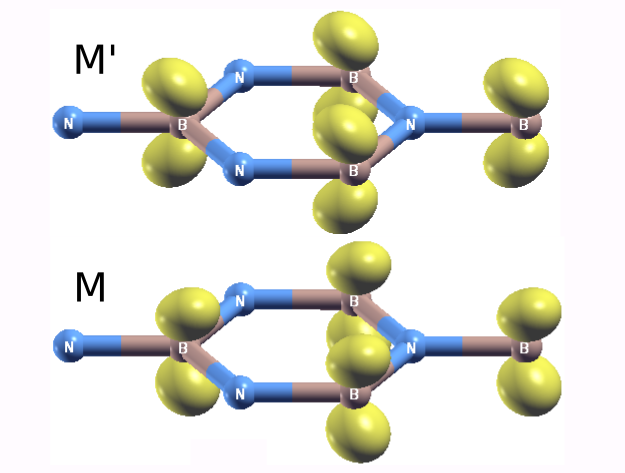
\includegraphics[width=0.4\textwidth]{M_and_M_prime.png}
	\caption{$\pi^*$ atomic-like orbitals of the conduction band minima on one of the layers for a compression of 0.5\%. At \MM', the components of the wavefunctions are oriented along the compressed B-N bond. At \MM, they are oriented along one of the other bonds.\textcolor{red}{Rajoute des flèches pour montrer le strain.}}
	\label{fig:WF_strain}
\end{wrapfigure}
The $\pi^*$ atomic-like orbitals at \MM~and \MM' have a different shape, as illustrated in Fig. \ref{fig:WF_strain} for a compression of 0.5\%. While they are degenerated in energy for the unstrained crystal, this degeneracy is lifted due to the symmetry breaking. The state with orbital components along the strained bond is the one whose energy changes with strain at \MM'. These orbitals are dependent on the interlayer interactions, which in turns depends on the interlayer distance. This distance varies linearly with the strain applied to the system in our relaxation process. This explains the splitting of the bands induced by strain at the \MM' point.

The valence states around \KK~and \KK' are only slightly changed in energy. This can be explained because the orbitals corresponding to these states are protected from interlayer interactions by symmetry, as shown in the theoretical study of Ref. \cite{kang2016unified}. There is nonetheless a slight change in energy, which causes the valence band maximum to be located at the point called \textbf{T}$_2$ under compression and at \textbf{T}$_1$ under stretch. \textcolor{red}{change the names either of these points OR of the T point in the BZ scheme}. The minimal indirect gaps are indicated by the dotted lines in Fig \textcolor{red}{Fig5} for compressive and tensile strain.

%
\section{Excitons and absorption}
On the low-energy end of the excitonic spectrum (in the sense of linear algebra) of bulk \acrshort{hBN}, we find two pairs of degenerate excitons. The splitting between the pairs is caused by the interlayer interactions and is called the Davydov splitting \cite{paleari2018excitons}. The two pairs transform differently under inversion operation (\textit{i.e.} taking $\rr \to -\rr$ or $\kk \to -\kk$). The lowest pair is even for inversion symmetry, which means it is dark in absorption. The second lowest pair instead is odd for inversion symmetry and thus bright. \textcolor{green}{have to explain what dark and bright is, somewhere} Note that this is true for one-photon absorption, at the linear response level. In non-linear optics, for instance two-photon absorption, the dark and bright characters are reversed. \\
The 120$\textdegree$ rotation symmetry breaking induced by uniaxial strain has an effect on the degeneracy of the Davydov pairs. First, looking at the energies of the four lowest excitons at $\Gamma$, as displayed in panel $(a)$ of Fig. \ref{fig:exc_abs_vs_strain}, we see that the energies are split, both for compression and stretching. 
These changes in energy are mainly due to the change in electronic gap reported in the above section. Indeed, they follow the same linear trend as the strain value increases and are of the same magnitude, about $\pm 0.1$ eV. We could also verify that the binding energies of the direct excitons remain approximately constant on the strain range considered, varying only by 10 to 15 meV.
\begin{figure}[h!tbp]
	\vspace{0.2cm}
	\setcapindent{2em}
	\centering
	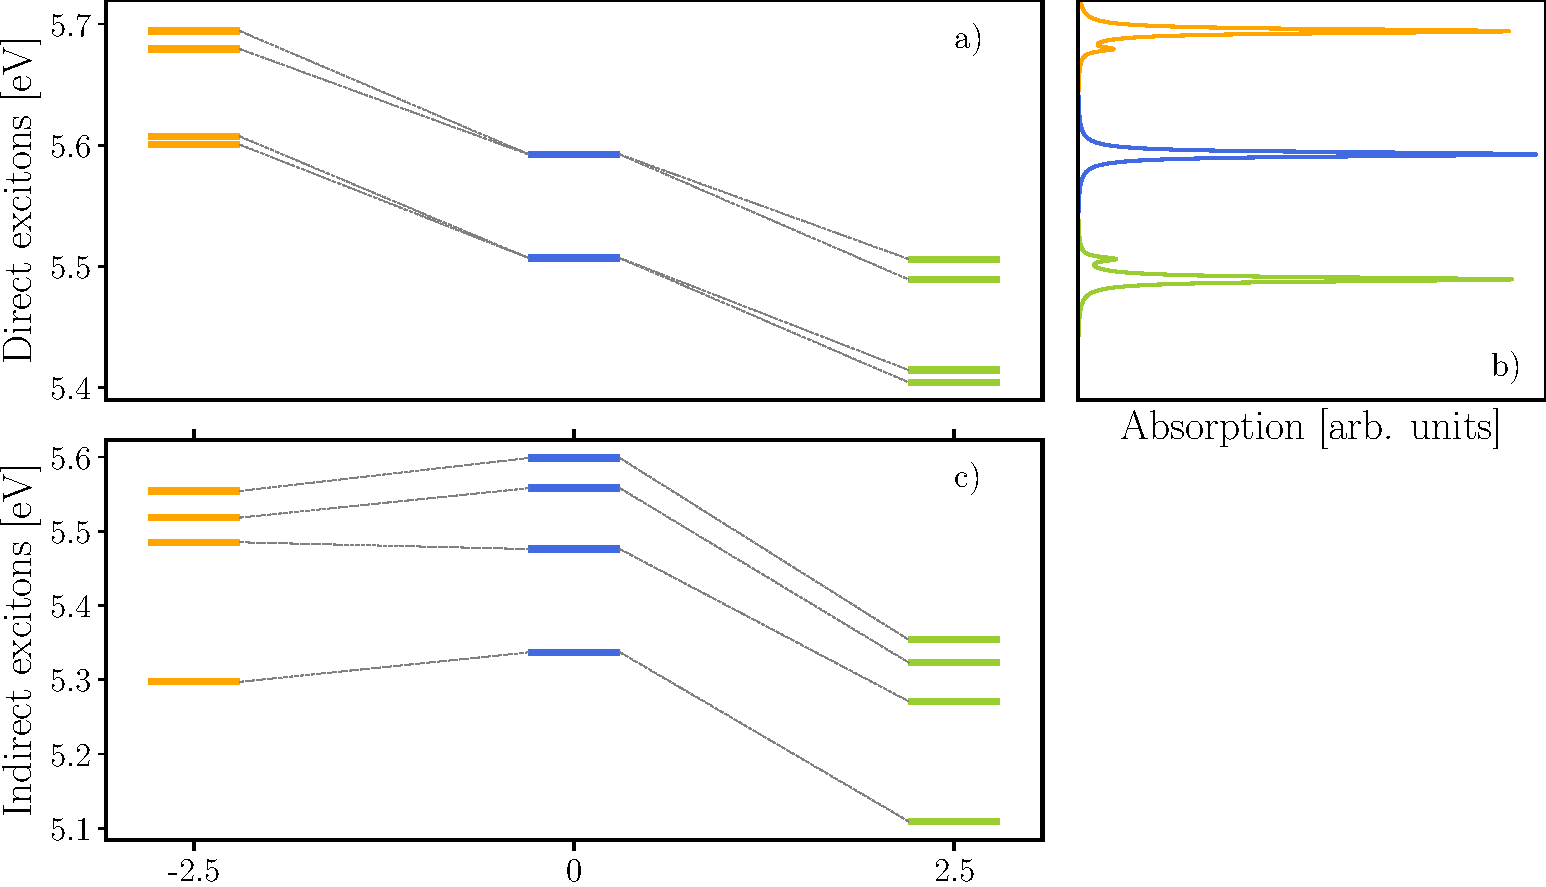
\includegraphics[width=0.8\textwidth]{hBN_exc_abs_vs_strain.pdf}
	\caption{\textcolor{red}{This also needs to change, and a trim please} Blue lines are for equilibrium crystal, orange is for compression and green is for stretch. (a) Energies of the lowest 4 excitons at $\Gamma$ (b) Absorption spectra associated with the direct excitons. Both excitons of the bright Davydov pair have a non-zero dipole matrix element and we can distinguish two peaks in the spectra for the strained crystals. (c) Energies of the lowest 4 indirect excitons.}
	\label{fig:exc_abs_vs_strain}
\end{figure}

The associated absorption spectra are displayed in panel (b) of Fig. \ref{fig:exc_abs_vs_strain}. As the inversion symmetry is not broken by uniaxial strain, the lowest two excitons remain dark when strain is applied. For the third and fourth lowest excitons in the strained systems, they are not mixed by the rotational symmetry as it is the case in the pristine crystal. This gives both excitons a non-zero dipole, and we see two peaks appearing in the absorption spectra. \\
The change of peak energy induced by strain is quantified by the strain gauge factor, which is defined as the spectral shift per \% of uniaxial strain. With these calculations, we find a value of $\approx$ 43 meV/\%, which is in the same range as transition metal dichalcogenides as reported in Ref. \cite{carrascoso2021strain}.

The splitting is also visible on the exciton wavefunctions in real space. It is displayed for the lowest two excitons at $\Gamma$, for a stretch of +2.5\%. The splitting is clear, with one of the wavefunctions having its components along the strained B-N bond or the armchair direction, while the other has its components along the zigzag direction.
\begin{figure}[h!tbp]
	\vspace{0.2cm}
	\setcapindent{2em}
	\centering
	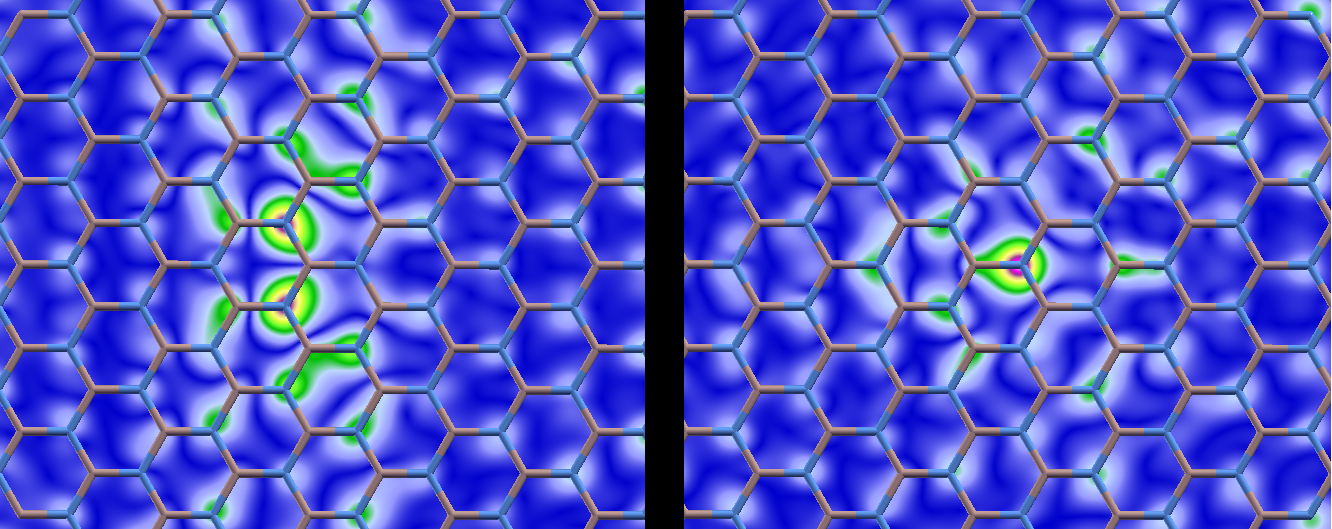
\includegraphics[width=0.8\textwidth]{excitonWF_strain.png}
	\caption{Electron distribution when the hole is fixed near the central Nitrogen atom, that we call exciton wavefunction. Left is the lowest dark exciton at $\Gamma$, right is the second lowest dark exciton at $\Gamma$, taken for a stretch of +2.5\%. \textcolor{red}{\textbf{IT seems that the hole is on the Boron here...}} }
	\label{fig:excWF_strain}
\end{figure}

We observe the same trend for the lowest-lying excitons with non-zero momentum, which we will call indirect excitons because they are formed by indirect electronic transitions. Their change in energy with strain is reported in Fig. \ref{fig:exc_abs_vs_strain} (c). It follows the same variation as the indirect gap and here again their binding energy is almost invariant with strain. The indirect excitons of hBN play an important role in light emission by luminescence. These changes in energy combined with the change in phonon frequencies will have an impact on the luminescence spectra of the strained crystals. This will be discussed in the next two sections.

%
\section{Exciton-phonon coupling from finite differences}
detail how we compute exc-ph coupling : numerical derivative of $\chi$ or of the exc dipoles  
spectra vs strain
mention excitonic temperature and Boltzmann population

We Taylor-expand the dielectric function with respect to atomic displacements. We neglect the variation of the delta in energy (this I need to explain (understand first lol)), so we are left with the derivative of the dipoles squared. We consider the minimal excitons which are dark, so the 0th order is 0. On the other hand, Taylor expanding the dipoles gives terms that will coincide only at 2nd order in atomic displacement (check the maths). All in all, it suffices to take 2nd derivative of dipoles, at 2nd order in atomic displacements. We compute this derivative numerically by finite differences (give formula here) : we displace atoms on one side, then the opposite side, BSE on each configuration, sum and boom. 


displacements with the scaling factor are converged to the value of 0.05 Angström. Needs to be big enough so the effect is bigger than numerical error, but small enough so that only the harmonic effects appear and not the higher order derivatives
%

As presented in the introduction of the thesis, the inclusion of lattice vibrations in our computational framework is necessary to describe accurately the phonon-assisted features in the luminescence spectrum of hBN. In particular the exciton-phonon coupling is the central quantity to take into account. To do so, I present in this section how to calculate the macroscopic dielectric function with a dynamical correction due to lattice vibrations, in a finite-difference scheme. \textcolor{green}{remember to cite FulvioPRL, Claudio}

We want to take the Taylor expansion of the response function with respect to atomic displacements around their equilibrium positions. We use the response function obtained from the \acrshort{BSE} without the long-range component so that the macroscopic dielectric function is readily obtainable following Eq. \eqref{eq:eps_macro}.
The contribution from exciton $\lambda$ to the response function  writes :
\begin{equation}
	\chi^\lambda_R(\omega) = \frac{|T^\lambda_R|^2}{E^\lambda_R - \omega + i \eta}
\end{equation}
where the subscript R indicates that the quantities are evaluated at clamped ion positions. The infinitesimal $\eta$ is taken independent of $R$ for simplicity. Here we recall that we define the exciton dipole matrix element $T^\lambda = \sum_{cvk} A_\lambda^{cvk} d_{cvk}$. The first derivative entering in the Taylor expansion will be :
\begin{equation}
	\frac{\partial \chi^\lambda_R(\omega)}{\partial R}\biggr|_{R=0} = \frac{\partial |T^\lambda_R|}{\partial R}\biggr|_{R=0} \frac{2|T^\lambda_{R=0}|}{E^\lambda_{R=0} - \omega + i\eta} + \frac{\partial \left[ E^\lambda_R - \omega + i\eta \right]^{-1}}{\partial R}\biggr|_{R=0} |T^\lambda_{R=0}|^2.
\end{equation}
This expression has a term linear in the exciton dipole and a term at the second power, both taken at clamped ion positions. It means that for dark excitons, the first derivative in the Taylor expansion will be zero. Excitons belonging in this category are labelled $\lambda'$, and we have $\frac{\partial \chi^{\lambda'}_R(\omega)}{\partial R}\bigr|_{R=0} = 0$
In \acrshort{hBN}, the excitons involved in luminescence are the ones which low at the lowest energies in the dispersion, at finite momentum. Because of momentum conservation, these ones cannot recombine and emit light which has almost zero momentum, hence they are dark at clamped ion positions. Phonons are needed to transfer momentum and assist their recombination. \\ 
Similar arguments hold for the second derivative in the Taylor expansion
and the only non-vanishing term that remains is :
\begin{equation}
	\frac{\partial^2 \chi^{\lambda'}_R(\omega)}{\partial R^2} = \frac{\partial^2 |T^{\lambda'}_R|^2}{\partial R^2}\biggr|_{R=0} \left[ E^{\lambda'}_{R=0} - \omega + i\eta \right]^{-1} \label{eq:chi_fdd}
\end{equation}
This derivative is evaluated numerically with the finite difference formula :
\begin{equation}
	\frac{\partial^2 \chi^{\lambda'}_R(\omega)}{\partial R^2} \approx \frac{\chi(\Delta\RR;\omega) - 2 \chi_0(\omega) + \chi(-\Delta\RR;\omega)}{\Delta\RR^2}
\end{equation}
Eq. \eqref{eq:chi_fdd} shows that it is equivalent to compute the finite-difference derivative of the full response function or only of the exciton dipoles. This is verified numerically in Ref. \cite{paleari2019exciton}

Switching focus to dielectric function rather that response function (they are linked by Eq. je sais plus combien), the Taylor exp is $\varepsilon \approx \varepsilon^{(0)} + \varepsilon^{st,(2)}_{\bar{q}}$. Static correction blabla, cite Zacharias Patrick Giustino. The second order is given by (Fulvio Eq. 3.38), avg over polariztion of light (because the lowest 2 excitons have different symmetries that will only allow coupling with certain phonon modes, in plane), restrict to momentum $\bar{q}$ where exc energies are minimal. (times 6 in a perfect BZ, times 4 in our case). Give thermal avg of atomic displacements (harmonic phonons). \textcolor{green}{this little paragraph could even be before the finite-difference derivation}. Now the Eq. 3.39, you can introduce the different processes : phonon abs and emission, giving different nominators. And finally Eq. 3.40. \\
Say how we compute the finite-diff deriv, supercells and displacing. Non-diagonal supercells \cite{Monserrat} : the minimum supercell size needed to fold a k-point at $\Gamma$ is the least common multiple of the Ni and not their product. Displacement of the atoms : Fulvio Eq. (B.3) 
Say that we use the W at eq positions for the displaced BSE. The \acrshort{RPA} static screening function is  interpolated from the unit cell. \\
vRS relation for luminescence. Temperature effects for the phonons are in the BE occupations (neglected for the strain article), for the excitons in the Boltzmann with excitonic temperature, Lorentzian model for broadening.



displace atoms, converge displacement, yambopy
\textcolor{red}{But now what happens to the displacement term in the Taylor expansion ? And include temperature aswell}
% supercells means folding of dark excitons at Gamma when atoms are clamped; they remain dark (verified numerically) and they acquire a momentum after displacing atoms (because of breaking of symmetries, derivative is non-zero etc)
% correction to the exciton energies due to exc-ph is neglected. Anyways we know that GW underestimates the gap so we won't have accurate energies. We are more interested in the shape of the spectra

%
\section{Luminescence results}
spectra vs strain, discussion

%
\section*{Conclusion of the chapter ?}